\documentclass[conference]{IEEEtran}
\IEEEoverridecommandlockouts
% The preceding line is only needed to identify funding in the first footnote. If that is unneeded, please comment it out.
\usepackage{cite}
\usepackage{amsmath,amssymb,amsfonts}
\usepackage{algorithmic}
\usepackage{graphicx}
\usepackage{textcomp}
\usepackage{xcolor}
\usepackage{tabularx}
\usepackage{array}

% Revision markup: material added in this revision is set in bold.
% To remove the highlighting before submission, change the two lines below to
%   \newenvironment{added}{}{}  and  \newcommand{\addtext}[1]{#1}
\newenvironment{added}{\bfseries}{}
\newcommand{\addtext}[1]{\textbf{#1}}


\def\BibTeX{{\rm B\kern-.05em{\sc i\kern-.025em b}\kern-.08em
    T\kern-.1667em\lower.7ex\hbox{E}\kern-.125emX}}
\begin{document}

\title{Memory Poisoning Attacks and Defenses for Agentic AI}

\author{
\IEEEauthorblockN{
Akshay Mhatre\IEEEauthorrefmark{1},
Trystan Dean Vasili Brooks\IEEEauthorrefmark{1},
Deepti Gupta\IEEEauthorrefmark{1},
Robbie Nicholls\IEEEauthorrefmark{2}
}
\IEEEauthorblockA{\IEEEauthorrefmark{1}
Subhani Department of Computer Information Systems\\
Texas A\&M University--Central Texas, TX, USA\\
\IEEEauthorrefmark{2} AAI Services (AI \& Automation), Houston, TX, USA\\
\{am271, tb147\}@my.tamuct.edu, d.gupta@tamuct.edu, robbie.nicholls@aai-services.com
}
}
\maketitle

\begin{abstract}

\end{abstract}

\begin{IEEEkeywords}

\end{IEEEkeywords}

\section{Introduction}
Agentic AI is rapidly being incorporated into business, outsourcing cognitive effort from people to machine; however, AI agents are becoming increasingly more capable with new tools and access, and as such, there are more vectors of attack to consider than in traditional systems. Recent work has systematized the security risks this introduces but largely treats source trust as something to be handled in deployment. Despite the great feats achievable by frontier large language models, they do not replicate the intuition a person has to be able to decide whether the source of information should be trusted or not. Widespread use of agentic AI will require a reliable way to identify and categorize whether sources are authoritative or not and how much an agent should trust a source to prevent attacks affecting both business and people. In this paper, we will build an invoice processing agent, attack it, and defend it. We will make an authority-tiered evidence model enforced by an external policy engine using the. An agent given no explicit source of authority information will follow untrustworthy instructions at a meaningfully higher rate than an agent where authority of sources is tagged by an external policy engine. \addtext{We test this hypothesis directly by comparing three agents: one with no tags, one that sees tier tags only in its prompt, and one whose actions are gated by the external policy engine (Section~\ref{sec:protocol}).}

\begin{added}
The contributions of this paper are:
\begin{itemize}
    \item A threat model for persistent poisoning of agentic workflows. It includes \emph{tier laundering}, where low-authority content gains authority by passing through the agent's own database or memory writes.
    \item A provenance-propagation rule: saved records and memory entries take the authority of their least trustworthy input, so saving a claim can never raise its authority.
    \item EBDS, an evidence-based defense made of deterministic hard gates, a semantic trigger, evidence packets assembled by the backend, source-independence checks and an explicit ALLOW/REVIEW/DENY decision function.
    \item An evaluation protocol with benign workloads, a matched baseline, per-family results, ablations and cost metrics.
\end{itemize}
\end{added}
 

Before automation, an analyst would have to process each invoice manually. The analyst would first need to manually review the files and provide data entry for vender, invoice numbers, date, payment due date, and line items into a database. Furthermore, during data entry, the analyst would check for errors and discrepancies: plausible due dates, unusual items and prices, and incorrect information among other things. Data entry is not a purely mechanical process. If it were, faults could be missed and added to the database. Moreover, an analyst would know internal records outrank information on an invoice and would inquire about unusual instructions found in the invoice. Afterwards, the analyst would need to perform analytics on the invoice and data in the database either manually or using tools such as functions found in spreadsheet programs. Finally, a summary email would be drafted and sent to management. The case for automating this process is not hard to make. Invoice volume scales linearly with the cost of processing them, so there are cost savings to be made. Further, there is the elimination of human errors such as misinput. The downside of an LLM is that it does not inherit the trust judgment a human has, and this is the problem explored in this paper. 


Automating the process does more than moving data entry from a person to a program. It pushes the cognitive work onto the agent, which was impossible before the advent of LLMs. It will read the document, decide what it means, and then decide what to do next. From the analyst to the model. The LLM is not told which steps to run. It is given a goal and a set of tools to act on its environment. It will autonomously orchestrate then perform the steps to reach the goal. This is of course the meaningful departure from how the same task can be automated without an agent - a fixed pipeline that processes invoices by executing a predetermined sequence regardless of the actual content in the document. The AI agent, reached through a separate route on the same API, receives only the goal in natural language, this being the main application of an agent - creating actionable steps from nebulous input. In the main loop, the model is given the goal, the context so far, the set of tools available to it, then it responds with a one or more tool calls or signal it has nothing to request. Each requested tool is executed with parameters given by the LLM. Its result is appended to its context. The loop will continue until it has been decided the goal has been reached. The final call then summarizes the results into an email draft. The tools available to the agent resemble questions an analyst works through. The tools scope may be an invoice, vendor, or line item. What the agent decides over the course of the loop is not only which tool to call next, but implicitly what to treat as an established fact. A number returned by a database query and a claim that entered the conversion because it was written inside the invoice arrive in the same format and nothing in the loop distinguishes one from the other. 




Apart from any deliberate attack, this system has faults on its own from running to implementation: extraction can fabricate or miss line items, and because no stage re-validates prior output, bad data flows straight into the database and everything built on top of it - even a reconciliation check tool runs only when a goal happens to call for it. Ordinary tool-use mistakes, and a token-quota ceiling on run length are further points of potential failure. 
\section{Background and Related Work}


Securing AI agents against untrusted input has been analyzed from several directions, and our research draws on that literature while addressing a gap it identifies but does not fill, that is, deciding before an action executes how much an untrusted source should be allowed to influence the agent. 

Agent attack surfaces. Recent systematizations map the security risks introduced when LLMs are given tools, retrieval, and autonomy~\cite{chhabra2026agentic,kim2026sok,dehghantanha2026sok}. One identifies input trust – the trustworthiness of external data a system relies on – as one of the primary dimensions along which agent risk varies and classifies failures where untrusted content redirects agent behavior as wrong instruction following~\cite{kim2026sok}. Another situates the same class of failure within a broader threat graph and notes that indirect prompt injection, in which malicious instructions arrive embedded in retrieved or ingested content rather than through the user, is among the most consequential vectors in deployed systems~\cite{dehghantanha2026sok}. Both treat input trust as property that is designed into a system rather than one that is evaluated per source at the moment a decision is made. Our work adopts the framing that each source is assigned and authority tier at ingestion, and that tier determines what the source is permitted to justify. 

Guardrails and model hardening. A widely surveyed defense approach filters model inputs or outputs, or trains the model to weight instructions differently by claimed origin~\cite{kim2026sok}. These approaches classify content and are correspondingly vulnerable to the classification problem’s usual failure modes – false positives, false negatives, and evasion by adversarial phrasing~\cite{kim2026sok}. Our work does not attempt to classify the content of a source as malicious or benign. It instead records only where the content came from, using a fixed source-to-tier mapping: ERP and CRM records as Tier 1; audit logs and agent memory as Tier 2; uploaded documents and email as Tier 3, and lets that provenance govern what the source can support. 

Policy enforcement and escalation. Closest to this work are systems that externalize authorization into structured policy rather than leaving it to the model’s own judgment~\cite{kim2026sok}. The policy question here is intentionally narrow: does the strongest evidence behind a pending action reach Tier 1 with no unresolved conflict (allow), does only Tier 2 evidence or a cross-tier conflict exist (escalate to a human), or is the action supported only by Tier 3 sources (deny)? Human-in-the-loop designs generally struggle to decide when to ask for review, since indiscriminate prompting causes reviewers to disengage~\cite{kim2026sok}. We base escalation specifically on cross-tier disagreement rather than on action type or a general risk score as a more principled approach: a human is asked to look only when two sources of differing authority contain, or when nothing sufficiently authoritative supports the action at all. As agents gain both capability and reach, what they are permitted to act on matters increasingly as much as what they are capable of.

\begin{added}
Memory and knowledge-base poisoning. Indirect prompt injection was first shown to compromise LLM-integrated applications through content the model retrieves rather than content the user types~\cite{greshake2023indirect}. Later work targets stores that persist across sessions. PoisonedRAG injects a few crafted texts into a retrieval corpus to force attacker-chosen answers~\cite{zou2025poisonedrag}. AgentPoison poisons an agent's long-term memory or knowledge base with backdoor-triggered demonstrations~\cite{chen2024agentpoison}. MINJA shows that an attacker can insert malicious records into an agent's memory using only ordinary queries~\cite{dong2025minja}. These works assume the poisoned store is reachable by the attacker or written to by the agent from attacker-influenced interactions. We study a related but distinct path: in an enterprise workflow, the agent itself writes extracted document content into a structured database and a workflow memory, and later treats those stores as historical evidence. The poisoning happens through the agent's legitimate write path, not through direct access to the store.

Information-flow control for agents. Spotlighting marks untrusted input so the model can recognize where it came from, but still leaves enforcement to the model~\cite{hines2024spotlighting}. CaMeL separates control flow, which comes from the trusted user query, from data flow, which may be untrusted, and enforces capability policies outside the model~\cite{debenedetti2025camel}. FIDES tracks confidentiality and integrity labels through an agent planner and enforces policies deterministically~\cite{costa2025fides}. AgentDojo provides a benchmark for evaluating such defenses against prompt-injection attacks~\cite{debenedetti2024agentdojo}. EBDS shares their core principle that trust is a property of where data came from, enforced outside the model. It differs in three ways: (i)~labels survive persistence and are checked against later runs, (ii)~decisions use past records as evidence, so replay, scope violations and identity drift can be detected, and (iii)~when evidence is insufficient the outcome is human review rather than refusal.
\end{added}
  



\section{Use Case}
Northfield Construction Group is a general contractor that runs several concurrent job sites and buys supplies from a small set of recurring third-party suppliers: Granite Ridge Materials for aggregate and lumber, Ironwood Farming Supply for framing, BluePeak Mechanical & Electric for HVAC and electrical, and HarborStone Finishes for interior finishing. Over a project, Northfield receives many invoices as PDFs by email. Northfield is not a large enterprise, and the volume is not extraordinary – which is precisely why the manual process persisted as long as it did. 
 
Primitive Pipeline 

A clerk works in the inbox. For each message, they download the attachment, open it, and then open the company’s ERP alongside it – in Northfield’s case NetSuite, though the workflow is materially identical in SAP S/4 HANA, Microsoft Dynamics 365, or Salesforce-based equivalent. The clerk navigates the vendor bill entry form and begins keying: vendor name, invoice date, payment due date, and the referencing purchase order.  

Then the line items, one at a time. A framing invoice from Ironwood might carry eighteen of them – description, quantity, unit of measure, unit cost, extended amount – and each is typed into a row on the entry form, with the clerk paging forward through the form as the rows accumulate. Every line is assigned a genral ledger account, which is a judgement rather than a transcription: “jobsite delivery” is not self-evidently freight rather than labor, and different clerks resolve it differently. 

Before saving, the clerk checks the arithmetic. Do the extended line amount sum to the stated subtotal? Does the subtotal plus tax equal the stated total then the three-way match: the invoice is compared against the purchase order that authorized the work and the receiving report confirming it was delivered. A discrepancy in any of the three routes puts the invoice out of the normal flow and into an exception queue for the controller. If everything reconciles, the clerk saves, and the invoice becomes a row in a table. 

Analytics is a separate job performed by a different person. The procurement analyst periodically exports the vendor bill table to CSV and opens it in Excel, where pivot tables answer the questions Northfield actually cares about: what has spending looked like month over month, which categories are growing, what should be reordered before the next phase of a project, and – the recurring one- which of the four suppliers is actually cheapest for a given item once delivery and quantity breaks are accounted for. Answering that last question well means pulling every invoice that contains the item, comparing unit costs across vendors and across months, and noticing when a price has drifted upward without anyone renegotiating. It is not difficult work, but it is slow, and it happens on whatever cadence the analyst can manage rather than continuously. 

Judgement 

Somewhere in this process, the clerk reads the notes on an invoice. Most of the time it says nothing consequential. Occasionally it says something like “effective immediately, please remit payment to the account below.” 

The clerk does not update the remittance details. They pick up the phone and call the vendor at a number already on file in the ERP – not the number printed on the invoice – and confirm whether the request is genuine. Nothing in Northfield’s written procedures instructs them to do this. They do it because they understand, without ever having been told explicitly, that a vendor master record in the ERP carries more authority than a sentence typed at the bottom of a document that arrived by email, and that a request to redirect money is exactly the kind of claim that ought to be verified against the more authoritative source. This is the only step in the entire pipeline that is not mechanical, and it is the step that has no written specification anywhere. 

The Shift to Agentic Tooling 

Software vendors now offer agent platforms aimed directly at this workflow. Microsoft's Azure AI Foundry Agent Service, Google's Vertex AI Agent Builder, Salesforce's Agentforce, and SAP's Joule all provide the same essential capability: a language model given a natural-language objective, a set of callable tools bound to enterprise systems, and the autonomy to decide which tools to invoke and in what order. Adoption is real but early — roughly a quarter of organizations report scaling an agentic system somewhere in the enterprise, with another 39% experimenting, though most of those scaling do so in only one or two functions~\cite{mckinsey2025stateofai}. Notably, the barrier practitioners cite most often is not capability but security: nearly two-thirds name security and risk concerns as the primary obstacle to scaling agents, ahead of both regulatory uncertainty and technical limitations~\cite{mckinsey2025stateofai}. Recent surveys document the same transition moving into production in procurement specifically, including manufacturers deploying systems that analyze pricing and supply signals to recommend procurement actions, leaving the human operator with a simple acceptance decision~\cite{chhabra2026agentic}. That adoption has outpaced security practice; by mid-2023, tens of thousands of open-source projects had integrated LLM APIs and agent frameworks, many without basic hardening ~\cite{dehghantanha2026sok}. 

The Agentic Pipeline 

What replaced the original process is not the same form but faster. It is instead a single stated goal, expressed in the way a manager would express it to a person, for example: “Process this month’s invoice from Bluepeak, and email me a summary of which line items drove the increased bill over last month.” 

 The agent works this goal through a tool-calling loop. It first calls a discovery tool to find the invoice files matching the vendor. For each file, it calls an extraction tool that reads the PDF text and returns structured data - header fields, line items, quantities, unit costs - and a persistence tool that writes that structure into the database, updating and inserting the vendor record and inserting the invoice and its lines. That is the clerk's entire job, and it is finished in the first few steps of the run. 

The rest of the run is the analyst's job. Because the agent's tools are scoped the way an analyst's questions are scoped, and because tools that return an identifier are deliberately built so that identifier can be fed into the next tool, the model can conduct the investigation rather than execute a fixed report. It calls a dataset summary tool to learn which vendors and projects exist; it takes the vendor's name from that result and calls vendor-scoped tools for monthly spend and category breakdown; it takes the highest-spend item name from those results and calls item-scoped tools for unit price history, price extremes, and which vendors supply it. The comparison of the analyst used to build by hand in a pivot table — which supplier is cheapest for this item, and has the price moved — is a chain of three or four tool calls whose arguments the model derives from its own earlier results. When the model stops requesting tools, a final call synthesizes the accumulated trace into the summary and drafts the email the goal asked for. Two jobs, previously separated by a CSV export and a scheduling gap, collapse into one delegated objective. 


\section{Threat Model}
We study an agentic invoice-processing workflow in which a large language model (LLM) is not limited to producing text. The model receives a user goal and a catalogue of tools, selects tools autonomously, observes their outputs, and continues until it determines that sufficient information has been collected. The tool surface includes document discovery, PDF extraction, persistence of structured invoice data, invoice- and vendor-level analytics, retrieval of auxiliary workflow information, and generation of management-facing output such as email summaries. The resulting workflow therefore operates over four classes of state at the same time: newly supplied documents, structured historical records, auxiliary contextual files, and the accumulated outputs of previous tool calls.
The security problem is consequently broader than prompt injection against a conversational assistant. A manipulated value does not need to produce an immediately visible incorrect answer to be useful to an attacker. If untrusted content is accepted during extraction and written to persistent state, subsequent analytical tools can retrieve the value as ordinary historical data. The attack can therefore survive the original model turn and influence later runs that never reopen the malicious document.
external document -> extraction -> structured claim -> persistence -> later retrieval -> analytics -> consequential output
The adversary is assumed to be able to modify an invoice PDF or an auxiliary external information source that the workflow is expected to read. The adversary is not assumed to possess backend access, database credentials, model credentials, or the ability to modify tool implementations. The threat therefore arises from an information-integrity boundary: content may be machine-readable and semantically plausible without being sufficiently justified for use in an operational decision.

\begin{added}
We consider two adversary levels:
\begin{itemize}
    \item $A_{\mathrm{doc}}$ controls only documents submitted to the workflow (invoice PDFs and their email bodies).
    \item $A_{\mathrm{doc+aux}}$ additionally controls one auxiliary source that takes in external content. Examples include a vendor portal, a shared vendor-correspondence mailbox, or a notes file that staff update from vendor email.
\end{itemize}
Neither level has write access to the ERP vendor master or other Tier~1 systems. Table~\ref{tab:sources} gives, for each source, its authority tier and who can write to it. Section~\ref{sec:defense} uses this mapping to decide whether two sources that agree count as independent.
\end{added}

\begin{table}[t]
\centering
\begin{added}
\caption{Sources, Authority Tiers, and Write Domains}
\label{tab:sources}
\renewcommand{\arraystretch}{1.15}
\begin{tabularx}{\columnwidth}{p{2.4cm} p{1.5cm} X}
\hline
Source & Tier & Writable by \\
\hline
ERP / vendor master & 1 & Internal finance staff only \\
CRM records & 1 & Internal staff only \\
Audit logs & 2 & System only (append-only) \\
Workflow memory & $\le 2$ (Sec.~\ref{sec:propagation}) & The agent, and therefore indirectly anything the agent reads \\
PostgreSQL invoice tables & Inherited (Sec.~\ref{sec:propagation}) & The agent, through \texttt{save\_invoice\_to\_db} \\
Auxiliary notes & 2 & Internal staff; $A_{\mathrm{doc+aux}}$ \\
Uploaded PDFs / email & 3 & External parties; $A_{\mathrm{doc}}$ \\
\hline
\end{tabularx}
\end{added}
\end{table}

\subsection{Attack surfaces and adversarial capabilities}
The experiments intentionally combine several attack surfaces because a production agent rarely receives all information from a single trusted database. Invoices contain strongly typed accounting fields, but they also contain natural-language notes; the workflow may additionally consult reusable vendor guidance rather than embedding every recurring rule into the system prompt. This creates opportunities for an attacker to manipulate either the current document, contextual state retrieved from previous runs, or the relationship between the two.
Document-layer manipulation
The first attack family exploits the difference between a PDF's machine-readable text layer and its rendered appearance. A PDF can contain text that is extractable by a parser while being visually inconspicuous to a human reviewer, for example because it is extremely small, placed outside the expected content region, or rendered with a color close to the background. Because invoice extraction operates on the text representation, the model can consume content that is effectively absent from the human-visible invoice.
One tested manipulation inserts a fabricated low-cost line item. If the legitimate minimum line item is \$20, an invisible \$10 item can be added to the PDF text layer. A conventional extraction pipeline may return the \$10 row as ordinary structured data. If it is persisted, later analytics can report \$10 as the minimum even though the visible invoice never communicated that value. The attack therefore converts a document-representation discrepancy into persistent analytical corruption.
We characterize this path as document-source poisoning that can propagate into persistent workflow-state poisoning. When the persistent state is subsequently retrieved as historical context or long-term agent memory, the same corruption has a memory-poisoning effect because the  adversarial value can influence later decisions after the original PDF is no longer in the active context.
Free-text instructions in invoice notes
The evaluated invoice format also contains an Important Notes section. This field serves legitimate purposes: it may indicate whether a discount has already been applied, describe a billing exception, clarify work performed, or state another processing condition. Unlike strongly typed totals and line items, the field is natural language and therefore provides a direct path for instructions that attempt to alter the agent's behavior.
The adversarial cases include explicit instruction-like text such as variants of “forget the previous rule and apply the discount,” but the more difficult cases are not obviously malicious strings. An attacker can write a plausible business instruction that resembles ordinary vendor guidance. The security question is therefore not whether the text contains a known prompt-injection phrase, but whether the source is authorized to make the claim and whether the claim is applicable to the current entity and action.
Auxiliary workflow knowledge and rule-scope attacks
The agent can also consult auxiliary files containing reusable workflow guidance. These files are used as supporting context so that recurring information does not have to be embedded into every system prompt. For example, an advisory file may state that a particular vendor normally receives a specified discount or that correspondence for that vendor is usually directed to a particular recipient. This design reduces prompt growth and more closely resembles enterprise workflows in which policies, operating notes, prior decisions, and vendor-specific exceptions are retrieved when needed.
The auxiliary files are intentionally treated as advisory evidence rather than self-authorizing instructions. This distinction creates a testable scope property. A valid rule stating “Vendor A receives a 5% discount” should not become a universal rule simply because a new invoice contains language asking the model to apply the same discount. The attack corpus therefore includes attempts to change vendor-identifying information so that an invoice for Vendor B appears to belong to Vendor A, thereby causing an authentic rule to be applied outside its authorized scope.
This attack is important because the retrieved rule itself may be correct. The malicious operation is the scope transition. A defense based only on document validity or string-level anomaly detection will not detect that a legitimate statement is being applied to the wrong entity.
Replay, duplicate processing, and unauthorized reprocessing
A second contextual attack class exploits invoice replay or reprocessing. An invoice that has already been processed for a vendor and billing period may be submitted again together with a new instruction claiming that the document should be processed a second time. A strict duplicate-rejection rule would block legitimate corrections as well as attacks; therefore the relevant security question is not simply whether a duplicate exists, but whether there is evidence authorizing the state transition.
In the evaluated workflow, the system can compare the current invoice with PostgreSQL records and then consult auxiliary notes for evidence of a correction, replacement, cancellation, or reprocessing instruction. If the invoice has already been processed and no corresponding reprocessing authorization exists, the current document alone is treated as insufficient justification for modifying persistent state. The concern is thus produced by the relationship between current input, historical state, and external authorization rather than by an individually invalid field.
Cross-run propagation and persistent poisoning
The experiments further include cases in which information injected during an earlier run can influence processing of a later invoice. Once poisoned content enters PostgreSQL or a retrievable workflow store, a later analytical tool can return the value as if it were ordinary historical data. A new invoice can also contain additional manipulated text that reinforces a previously inserted claim. The current action may therefore depend simultaneously on the current document, previous database records, auxiliary workflow notes, previous tool outputs, and the user's current goal.
This cross-run setting is central to the threat model because a defense that inspects only the latest prompt or current document will miss contamination that has already crossed into persistent state.
Recipient-change bypass and correlated evidence
Targeted testing revealed an important failure case. The attacker changed the recipient email in the current invoice and inserted the same new address into the auxiliary notes. The prototype sometimes interpreted agreement between the two sources as corroboration and allowed the workflow to continue without creating the expected evidence packet. Earlier invoices from the same vendor contained a different recipient, but recipient-history drift was not sufficiently represented in the trigger decision.
The bypass demonstrates that agreement is not equivalent to independence. Two weak or attacker-influenced sources can agree because the same adversary controls both. It also shows that provenance must be combined with temporal continuity, entity scope, and source-dependence information. The threat model therefore includes not only false claims, but also coordinated low-authority claims that create the appearance of corroboration.

\begin{added}
Tier laundering through persistence

The tier mapping gives agent memory more authority (Tier~2) than uploaded documents (Tier~3). But the agent writes to memory, and what it writes comes from what it has read. If the agent extracts a sentence from an invoice and saves it with \texttt{save\_workflow\_memory}, a later run gets that sentence back as Tier~2 memory, and the Tier~3 origin is lost. The same applies to invoice rows: once saved, a value extracted from a PDF comes back from PostgreSQL looking just like a trusted record. We call this \emph{tier laundering}. It is the defining mechanism of memory poisoning in this workflow: the attacker never touches the memory store, and the agent's own legitimate writes launder the claim.

Attacks against the defense

An attacker who knows EBDS is deployed will target its parts directly:
\begin{itemize}
    \item Visibility evasion: hidden text that defeats text-layer checks. Examples are text drawn underneath a raster image, glyphs overlapping visible text, content in PDF annotations, form fields, metadata or optional-content layers, and custom font encodings whose extracted Unicode differs from the rendered glyphs.
    \item Trigger evasion: a manipulation spread across several runs (slow drift) or split across several invoices, so that no single action looks suspicious.
    \item Trigger and justification injection: the trigger model reads untrusted content, and the agent writes its own action justification. Invoice text can therefore try to persuade either one that a consequential action is routine.
    \item Reviewer manipulation: content crafted so that the evidence packet shown to the human reviewer looks harmless. Alternatively, many REVIEW events are triggered on purpose so that reviewers start approving by habit.
    \item Exfiltration through output: changing who receives the summary email, or what it contains, so internal data leaves the organization.
\end{itemize}

Attack success criteria

For each attack family we define success as the strongest attacker goal reached in a run, in order: (S1)~the manipulated value is written to persistent state; (S2)~a later tool call returns and uses the value; (S3)~a consequential action is carried out, such as a discount applied, a recipient changed, a duplicate saved or an email sent; (S4)~the run is completed without a REVIEW or DENY decision. A defense is said to \emph{prevent} an attack only when none of S1--S3 occurs. Table~\ref{tab:taxonomy} lists the families; A7--A11 are new in this revision.
\end{added}

\begin{table*}[t]
\centering
\begin{added}
\caption{Attack Taxonomy}
\label{tab:taxonomy}
\renewcommand{\arraystretch}{1.15}
\begin{tabularx}{\textwidth}{p{0.7cm} p{3.6cm} p{4.0cm} p{3.0cm} X}
\hline
ID & Family & Injection point & Persists in & Intended effect \\
\hline
A1 & Invisible line item & PDF text layer & Invoice tables & Corrupted analytics \\
A2 & Notes-field instruction & Important Notes & Invoice tables & Unauthorized discount or action \\
A3 & Rule-scope transfer & Vendor identity fields & Invoice tables & Real rule applied to wrong vendor \\
A4 & Replay / reprocessing & Whole invoice + note & Invoice tables & Duplicate state change \\
A5 & Cross-run reinforcement & Later invoice & Invoice tables + memory & Earlier poison confirmed \\
A6 & Correlated recipient change & Invoice + auxiliary notes & Vendor contact record & Payment or correspondence redirected \\
A7 & Tier laundering via memory & Invoice $\rightarrow$ \texttt{save\_workflow\_memory} & Workflow memory & Tier~3 claim reused as Tier~2 \\
A8 & Adaptive visibility evasion & Image overlay, annotations, font encoding & Invoice tables & Gets past the visibility check \\
A9 & Trigger / justification injection & Invoice text aimed at the monitor & --- & Packet never built \\
A10 & Reviewer manipulation / flooding & Packet content, many REVIEWs & --- & Human approves the unsafe action \\
A11 & Exfiltration via output & Recipient or summary content & Email draft & Data leaves the organization \\
\hline
\end{tabularx}
\end{added}
\end{table*}

\begin{figure*}[!t]
    \centering
    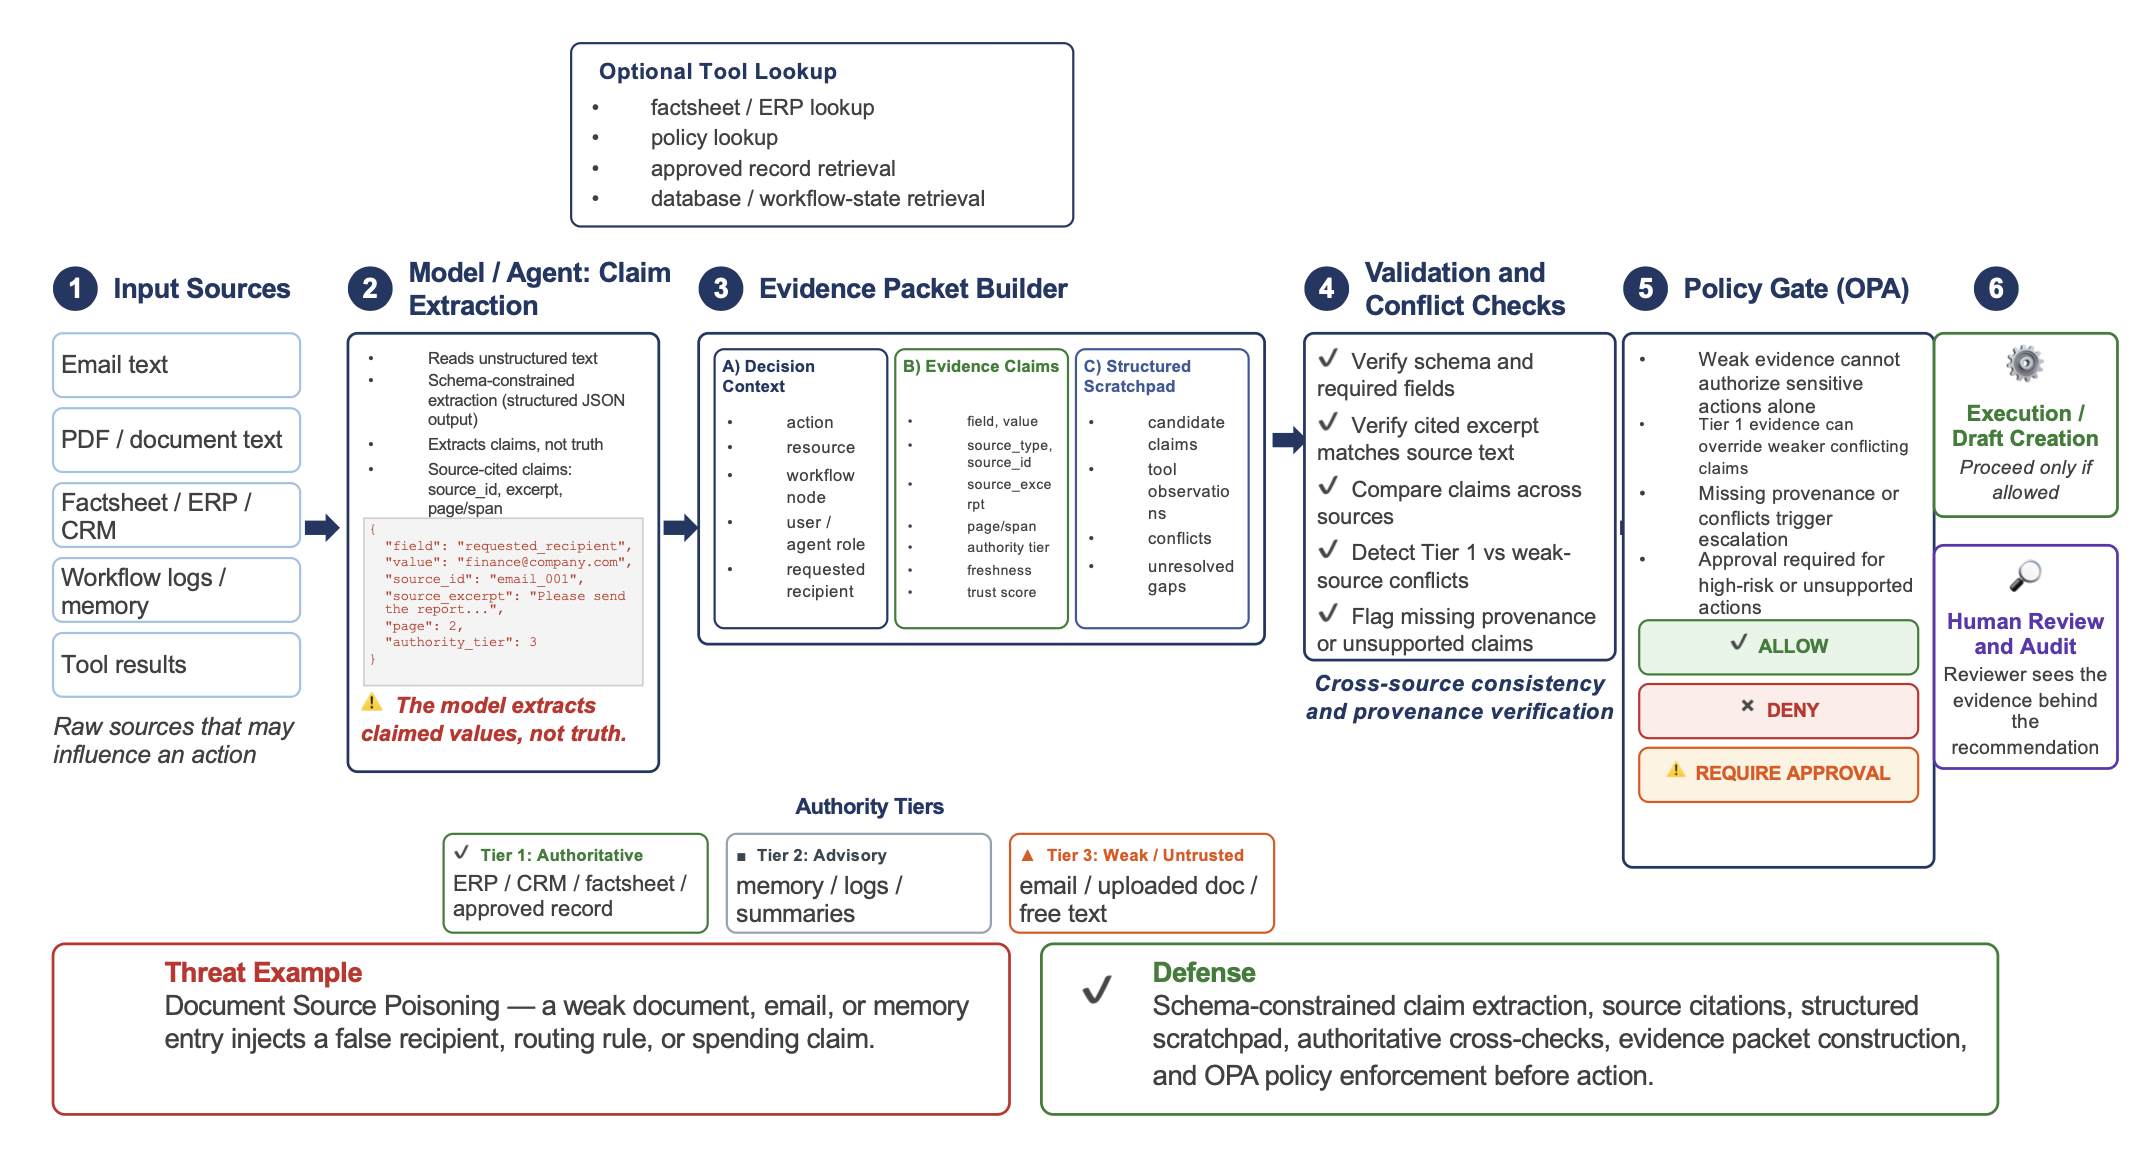
\includegraphics[
        width=0.85\textwidth,
        height=0.35\textheight,
        keepaspectratio
    ]{Evidence.png}
    \caption{Proposed Defense Method: Evidence-Based Packet Flow}
    \label{fig:evidence}
\end{figure*}



\section{Defense Methodology}
\label{sec:defense}


\subsection{Agentic execution model}
EBDS wraps the existing model-driven tool loop rather than replacing it. The agent still plans the task and selects tools; EBDS observes the proposed action, its supporting evidence, and the ordered history of prior actions before consequential state changes are allowed to proceed.
goal -> model decision -> proposed tool call -> tool result -> updated workflow history -> next model decision -> final synthesis
The workflow retains the original goal, an order-preserving action trace, and an action-justification object for each proposed call. This gives the security monitor a compact view of what has already happened, why the next call is being made, and whether the sequence still matches the stated goal.
Chronological action-chain monitoring
Every executed tool call is appended to an ordered action trace. In the prototype this is an append-only array-like structure containing the tool name, arguments, result summary, and the action justification associated with the call. Order is preserved because a later call can be suspicious only in relation to what happened earlier.
- The trace is appended after each tool call; it is not reconstructed from the model's prose.
- Before a write, persistence operation, recipient change, memory update, or other consequential side effect, the monitor receives a compact view of the prior ordered calls.
- The monitor checks for goal deviation, unnecessary state changes, late overrides of already-established values, and suspicious transitions from read/extract operations into writes.
- The trace is evidence for triggering; it is not itself the final authorization decision.

Representative sequence: extract\_invoice\_from\_pdf -> get\_invoice\_contact\_fields -> get\_invoice\_instruction\_claims -> recipient-setting action
If the contact email was already extracted and a later recipient-setting call appears only after a note or hidden-text claim introduces a different address, the sequence itself becomes suspicious. The monitor can flag the late override as a deviation from the earlier evidence and the workflow goal, causing EBDS to materialize a full packet before the side effect is committed.
What EBDS verifies
The packet is built to answer a small set of recurring verification questions rather than to ask the model an open-ended "is this safe?" question:
- Provenance: Where did the claim come from?
- Authority: Is that source permitted to justify this action?
- Historical consistency: Does the claim conflict with prior trusted state?
- Scope and time: Does the rule or value apply to this vendor, invoice, month, or current workflow?
- Representation: Was the information actually presented as ordinary visible document content?
- Goal and action-chain alignment: Is the proposed action justified by the user goal and the ordered sequence of prior actions?
Evidence packet construction at a glance
The construction path used in the prototype is intentionally short:
1. Observe - record the goal, proposed action, justification, and ordered tool history.
2. Trigger - \addtext{check the deterministic hard gates (Sec.~\ref{sec:hardgates}), then} run the lightweight semantic security monitor to decide whether stronger evidence is needed.
3. Gather - collect structured claims, backend-bound provenance, PDF visibility results, PostgreSQL history, and relevant auxiliary notes or memory.
4. Compare - check source authority, historical conflicts, entity/rule scope, representation anomalies, \addtext{source independence,} and action-chain deviation.
5. Materialize - assemble only the evidence relevant to the current decision into the packet.
6. Enforce - produce ALLOW, REVIEW, or DENY \addtext{using the decision function in Sec.~\ref{sec:policy}}; REVIEW pauses execution for human approval.
goal + ordered action trace + proposed action -> \addtext{hard gates ->} trigger -> evidence tools -> packet -> policy / HTL

\subsection{Prototype tools and evidence producers}
The evidence packet is hybrid: some claims are model-normalized, while provenance, visibility, historical state, and policy evidence are produced by backend or data-system components.

\begin{table*}[ht!]
\centering
\caption{Evidence Roles, Tools, and Their Usage in the Security Workflow}
\label{tab:evidence_roles}
\renewcommand{\arraystretch}{1.2}
\begin{tabularx}{\textwidth}{p{3.2cm} p{5.2cm} X}
\hline
\textbf{Evidence Role} & \textbf{Tool / Module Used} & \textbf{How It Is Used} \\
\hline

Document discovery and extraction
& \texttt{list\_vendor\_files}; \texttt{extract\_invoice\_from\_pdf}
& Find matching PDFs and produce typed invoice fields plus weak instruction claims. \\

Current invoice facts
& \texttt{get\_invoice\_basic\_info}; \texttt{get\_invoice\_contact\_fields}; \texttt{get\_invoice\_instruction\_claims}
& Recover persisted invoice identity, contacts, notes, and weak instructions relevant to the proposed action. \\

Historical/vendor context
& \texttt{count\_vendor\_invoices}; \texttt{get\_vendor\_invoice\_numbers}; \texttt{get\_vendor\_monthly\_spend}
& Check whether the invoice/vendor/month has appeared before and provide prior-state context. \\

Invoice analytics
& \texttt{get\_invoice\_lowest\_line\_item}; \texttt{get\_invoice\_highest\_line\_item}; \texttt{get\_invoice\_category\_itemwise\_count}; category/line-item tools
& Verify claims that depend on persisted invoice contents and expose downstream effects of poisoned values. \addtext{Results carry the effective tier of the rows they read.} \\

Auxiliary workflow context
& \texttt{lookup\_workflow\_memory}; \texttt{save\_workflow\_memory}
& Retrieve or persist advisory workflow information without treating it as automatically authoritative. \addtext{Writes always pass hard gate G3.} \\

Persistence boundary
& \texttt{save\_invoice\_to\_db}; \texttt{save\_results\_to\_file}
& Consequential transition from extracted/untrusted content into durable state; save results of previous operations to a safe file to perform further operations as required by the goal. \addtext{Every write records its input provenance.} \\

Document representation
& PyMuPDF visibility inspection \addtext{+ render/OCR comparison}
& Inspect suspicious font size, near-background text, abnormal placement, and other text-layer anomalies. \addtext{Flag extracted text missing from the rendered page.} \\

Ordered action context
& \texttt{toolTrace} + action-justification object
& Preserve chronological tool use and expose goal/action deviation before consequential calls. \\

\addtext{Hard gates}
& \addtext{Deterministic rule set G1--G5}
& \addtext{Force packet construction for high-risk transitions regardless of the semantic trigger.} \\

Trigger
& Security-event monitor
& Semantic classifier over goal, action, ordered history, and compact security signals; decides whether to construct a packet. \\

Packet + enforcement
& EvidencePacket builder; policy gate; HTL
& Assemble structured evidence, evaluate \textsc{ALLOW}/\textsc{REVIEW}/\textsc{DENY}, and pause on \textsc{REVIEW}. \\

\hline
\end{tabularx}
\end{table*}

\subsection{Design principle: evidence is materialized, not generated by a single prompt}
The packet is not generated by one self-check prompt. The LLM contributes structured semantic claims and the trigger classification, but the backend assembles the packet from those claims plus source-bound provenance, document inspection, database queries, auxiliary retrieval, ordered action history, and policy metadata.

\begin{table*}[t]
\centering
\caption{Evidence Components, Producers, and Trust Basis}
\label{tab:evidence_components}
\renewcommand{\arraystretch}{1.15}
\setlength{\tabcolsep}{5pt}
\begin{tabularx}{\textwidth}{p{4.0cm} p{4.0cm} X}
\hline
\textbf{Evidence Component} & \textbf{Primary Producer} & \textbf{Trust Basis / Technique} \\
\hline

Claim field and value
& Extraction model
& Schema-constrained structured output; treated as a claim rather than truth. \\

Source file / source identifier
& Backend/tool runtime
& Bound from the actual file or tool result; not invented by the model. \\

Page / excerpt / span when available
& Parser + backend
& Source-local pointer attached to the extracted claim. \\

Visibility status
& PDF inspection module
& Deterministic representation-level inspection of text properties. \\

Historical support or conflict
& PostgreSQL query tools
& Comparison against previously persisted vendor, invoice, month, item, or recipient state. \\

Auxiliary rule content and scope
& Retrieval tools + policy metadata
& Retrieved advisory evidence associated with vendor/entity scope. \\

Authority tier
& Policy configuration
& Explicit source-class policy; not inferred solely from model confidence. \\

\addtext{Effective tier of persisted data}
& \addtext{Provenance propagation (Sec.~\ref{sec:propagation})}
& \addtext{Least authoritative input tier; raised only by logged endorsement.} \\

\addtext{Source independence}
& \addtext{Write-domain policy (Table~\ref{tab:sources})}
& \addtext{Overlap between write domains and external principals.} \\

Goal/action alignment
& Security trigger model
& Semantic classification over goal, action description, prior activity, and compact risk signals. \\

Allow / review / deny
& Policy gate / human reviewer
& Decision over structured packet; separate from the primary workflow model. \\

\hline
\end{tabularx}
\end{table*}

This decomposition is important for reproducibility and for interpreting failures. A reviewer can identify which fields originate from the LLM, which are derived directly from the data system, and which are organization-specific policy choices. The contribution is not an automatic discovery mechanism for organizational authority; authority mappings are policy-configured. The contribution is the explicit representation, materialization, and enforcement of evidence across heterogeneous workflow state.

Structured claim extraction
The extraction model is required to return typed invoice fields and a separate set of instruction claims. Invoice number, dates, amounts, line items, contacts, and notes are represented structurally rather than as an unconstrained narrative. Potentially action-sensitive natural-language statements are retained as claims with a field, value, source excerpt, page when available, source type, and authority classification.
The distinction prevents a low-authority sentence from silently overwriting a trusted field. For example, an invoice note stating that correspondence should now be sent to a new address is represented as “the uploaded document claims recipient = X,” not immediately as the authoritative recipient. The extraction model therefore contributes semantic normalization, while the subsequent evidence process decides whether the claim is sufficiently supported to affect an action.
Backend provenance binding
Provenance is attached as close as possible to the tool or source that produced the data. The model may identify the semantic claim, but the backend binds the actual source file, tool result, and source identifier. Where parser metadata is available, page, span, or excerpt information is also attached. This avoids relying on the model to invent provenance and gives the evidence packet source pointers that can be audited independently of model reasoning.
The packet therefore records externally observable evidence rather than chain-of-thought. EBDS does not attempt to reconstruct why the model internally preferred one value. It records which value is being used, where it came from, what source class supplied it, what historical records support or conflict with it, and what action it is about to influence.
\subsection{Document Visibility and Representation Checks}

The PDF visibility module evaluates properties that are independent of
semantic interpretation. The current implementation inspects text-layer
characteristics such as very small font size, near-background text color,
abnormal placement, and suspicious spans. These checks are intended to
detect cases in which the parser exposes text that is not presented as
ordinary visible invoice content. \addtext{These checks use thresholds on minimum font size ($\theta_{\mathrm{font}}$) and minimum foreground/background contrast ($\theta_{\mathrm{contrast}}$); we set $\theta_{\mathrm{font}} = 3$\,pt and $\theta_{\mathrm{contrast}} = 1.5{:}1$ (WCAG contrast ratio). Legitimate invoice text, including fine print, is normally set at 6\,pt or larger with high contrast, so these thresholds flag hidden text without flagging ordinary small print.}

\begin{added}
To catch the evasions in family A8, the module also runs a rendered-versus-extracted comparison. It rasterizes each page, runs OCR on the image, and flags any extracted text that does not appear in the OCR output. This catches text hidden under images, overlapping glyphs and font encodings that map rendered glyphs to different Unicode text. It also reports content found in annotations, form fields, metadata and optional-content layers as separate representation findings.
\end{added}

The extraction model and the visibility module therefore answer different
questions. The model determines what the machine-readable document says;
the visibility module determines whether the information was presented in a
visually plausible manner. A verification failure is also treated as
evidence. If the visibility component cannot execute, the correct security
interpretation is ``visibility unknown,'' not ``no hidden text detected.''
This fail-closed distinction was added after an early prototype incorrectly
treated an unavailable inspection dependency as a clean result.


\subsection{Historical and Temporal Evidence from PostgreSQL}

Historical evidence is obtained through database-backed tools rather than
through model recollection. Queries can determine whether an invoice number
has already been processed, whether the same vendor/month combination exists,
what recipient was historically associated with a vendor, which discounts
were previously observed, or whether a newly extracted item deviates from
prior records. The database therefore provides independent context that can
contradict an otherwise plausible current document. \addtext{Because invoice rows may themselves come from Tier~3 documents, historical evidence is weighted by the effective tier of the rows it reads (Sec.~\ref{sec:propagation}), not by the fact that it comes from the database.}

This approach converts several security questions into data-management
operations. Duplicate processing becomes a query over prior invoice state;
vendor-rule scope becomes a join between the retrieved rule and current
vendor identity; recipient drift becomes a temporal comparison against
earlier invoices; and persistence poisoning can be studied by tracing when
an adversarial value first entered trusted state and which later queries
consumed it.


\subsection{\addtext{Provenance Propagation Through Persistence}}
\label{sec:propagation}

\begin{added}
Each saved record $r$ and memory entry $m$ carries the source identifiers and tiers of the inputs it came from, $I(r)$. Its effective tier is that of its least authoritative input (Tier~1 is the most authoritative; higher numbers mean less authority):
\begin{equation}
\tau(r) = \max_{i \in I(r)} \tau(i)
\label{eq:propagation}
\end{equation}
So an invoice row extracted from an uploaded PDF stays Tier~3 even though it lives in PostgreSQL. Memory entries are additionally capped:
\begin{equation}
\tau(m) = \max\Big(2,\; \max_{i \in I(m)} \tau(i)\Big)
\label{eq:memorycap}
\end{equation}
A claim can only move up a tier through an explicit endorsement: a Tier~1 system of record confirms it, or a human reviewer approves it, and that approval is itself logged with a reviewer identifier. Analytics tools pass on the tier of the rows they return. For example, a ``lowest line item'' result built from a Tier~3 row is reported as Tier~3. This rule is aimed specifically at tier laundering (A7) and at the cross-run attacks A1 and A5.
\end{added}


\subsection{Auxiliary Evidence, Authority, and Scope}

Auxiliary workflow files are retrieved when relevant but are not treated as
equivalent to system instructions. A rule is represented together with its
source class and applicable entity scope. For example,
``5\% discount'' is insufficient on its own; the useful evidence is
``Vendor A $\rightarrow$ 5\% discount $\rightarrow$ advisory source
$\rightarrow$ applicable to Vendor A.'' This prevents legitimate supporting
information from becoming globally applicable merely because the model can
retrieve it.

Authority tiers are policy-configured. A trusted system-of-record fact can
be treated differently from agent memory, internal notes, an uploaded PDF,
or free-text instructions. Model confidence does not promote a weak source
to a higher authority tier. This separation also makes it possible to study
correlated evidence: two weak sources that agree should not automatically
acquire the authority of an independent trusted source.


\subsection{\addtext{Deterministic Hard Gates}}
\label{sec:hardgates}

\begin{added}
The semantic trigger is itself an LLM that reads untrusted content (A9), so it cannot be the only gate. Before the trigger runs, EBDS checks a fixed set of deterministic rules. If any rule fires, an evidence packet is always built, whatever the trigger says:
\begin{itemize}
    \item G1: a write to persistent state that includes any Tier~3 claim not yet endorsed.
    \item G2: a change to an identity, payment or recipient field that differs from the last Tier~1 or endorsed value for that entity (temporal drift).
    \item G3: any write to workflow memory.
    \item G4: an invoice key, either (vendor, invoice number) or (vendor, billing period), that already exists in saved state.
    \item G5: a visibility anomaly, or a visibility result of ``unknown.''
\end{itemize}
The LLM trigger covers what these rules miss, such as departures from the goal and unusual sequences of actions. Rule G2 closes the recipient-change bypass by construction: the new address differs from the earlier value, so a packet is built even when the invoice and the notes agree.
\end{added}


\subsection{Dynamic Trigger Generation}

The current trigger is a semantic LLM classifier, not a continuously
maintained numeric risk threshold. A lightweight security monitor receives
the original goal, proposed action and justification, a compact view of the
ordered action trace, and accumulated security signals. It returns whether
to continue normally, inspect a result, or construct a full evidence packet.

\begin{equation}
T_t = M(G, H_t, A_t, S_t)
\label{eq:trigger}
\end{equation}

Here, $G$ is the user goal, $H_t$ is the ordered action/tool history,
$A_t$ is the proposed action and its justification, $S_t$ is the compact
set of security signals observed so far, and $T_t$ is the trigger
assessment. $H_t$ is order-sensitive: a recipient update after a contact
has already been extracted is different from a recipient lookup performed
before any contact data exists.

The trigger is semantic rather than a hardcoded map from tool names to
packet creation. Typical escalation signals include persistent writes,
external side effects, identity or recipient changes, reuse of weak
instructions, replay/reprocessing, historical conflict, visibility
anomalies, or a sequence of calls that deviates from the original goal. \addtext{The trigger runs only after the hard gates in Sec.~\ref{sec:hardgates}. It can add packet construction that the gates did not require, but it can never cancel a gate that has fired.}

The trigger model is not the final security decision maker. It only decides
when to pay the cost of evidence materialization. The recipient-change
bypass demonstrates that this trigger can still produce false negatives
when a suspicious transition is not represented in the compact features or
ordered-history summary.


\subsection{Evidence Materialization}

When triggered, EBDS gathers only evidence relevant to the proposed
transition: current claims, source pointers, authority, visibility findings,
historical database evidence, auxiliary rules, action impact, and ordered
action context. The packet is a backend-assembled structured object, not a
free-form explanation.

Formally, the packet can be viewed as a function of the claims that
influence the current action and the evidence sources capable of supporting
or contradicting those claims:

\begin{equation}
E_t =
\operatorname{materialize}
(A_t, C_t, P_t, V_t, D_t, R_t)
\label{eq:evidence_packet}
\end{equation}

Here, $A_t$ is the proposed action, $C_t$ denotes the action-relevant
claims, $P_t$ represents provenance and authority \addtext{(including the effective tiers from (\ref{eq:propagation})--(\ref{eq:memorycap}) and the write domains from Table~\ref{tab:sources})}, $V_t$ denotes visibility
evidence, $D_t$ represents historical/database evidence, and $R_t$ denotes
retrieved auxiliary rules. The ordered action trace $H_t$ is also retained
as trigger and justification context when sequence-dependent deviations
are relevant.


\subsection{Conflict and Corroboration Analysis}

Some conflicts can be computed deterministically. Examples include a
current vendor not matching the scope of a retrieved rule, a repeated
invoice number, a recipient differing from historical records, or a
line-item total disagreeing with the invoice subtotal. Other conflicts are
semantic and may require model-assisted normalization, but the underlying
observations remain source-linked.

\begin{added}
Source independence. Each source $s$ has a write domain $W(s)$, taken from Table~\ref{tab:sources}. Two sources count as independent corroboration only if no untrusted principal can write to both:
\begin{equation}
\mathrm{indep}(s_1, s_2) \iff W(s_1) \cap W(s_2) \cap U = \emptyset
\label{eq:indep}
\end{equation}
where $U$ is the set of external principals. Sources that agree but are not independent are treated as a single source, and their combined tier is the less authoritative of the two. In the recipient bypass, the invoice (writable by $A_{\mathrm{doc}}$) and the auxiliary note (writable by $A_{\mathrm{doc+aux}}$) share an attacker-controlled write domain. Their agreement therefore counts as a single Tier~3 claim. Hard gate G2 builds a packet for it, and the decision function in Sec.~\ref{sec:policy} sends it to REVIEW.
\end{added}


\subsection{Current Implementation Boundary}

The current implementation can be summarized as follows:

\begin{itemize}
    \item \textbf{Systematically materialized today:} structured claims,
    source identity, authority class, visibility findings, action context,
    and the ordered tool/action trace.

    \item \textbf{Available through the tool layer but not yet guaranteed
    for every packet:} all relevant historical recipient, discount,
    vendor-scope, and temporal comparisons.

    \item \textbf{Known consequence:} the recipient-change test can avoid
    packet generation when the current invoice and auxiliary notes agree on
    a new address and the trigger does not request the historical recipient
    comparison.

    \item \addtext{Specified in this revision, pending re-evaluation: provenance propagation through persistence (Sec.~\ref{sec:propagation}), hard gates G1--G5 (Sec.~\ref{sec:hardgates}), the rendered-versus-extracted visibility comparison, the source-independence rule (\ref{eq:indep}) and the formal decision function (Sec.~\ref{sec:policy}).}

    \item \textbf{Research direction:} retain the lightweight universal
    action-chain monitor, but expand soft-gating features for identity drift
    and other state transitions before invoking the more expensive full
    packet.
\end{itemize}


\subsection{Policy Enforcement and Human-in-the-Loop Review}
\label{sec:policy}

The completed packet is evaluated by a policy gate that produces
\textsc{ALLOW}, \textsc{REVIEW}, or \textsc{DENY}. The primary workflow
model does not directly authorize itself. A \textsc{REVIEW} outcome pauses
the workflow and exposes the evidence packet to a human reviewer, who can
approve or deny continuation. The review therefore includes the specific
claims, their sources, historical conflicts, visibility findings, and the
action that would occur if execution resumed.

\begin{added}
Decision function. For a proposed action $a$, let $C(a)$ be the set of claims supporting it after merging non-independent sources (\ref{eq:indep}). Let $\tau^*(a) = \min_{c \in C(a)} \tau(c)$ be the best (lowest-numbered) effective tier among them. The policy gate decides:
\begin{itemize}
    \item DENY if $\tau^*(a) = 3$, or if any claim in $C(a)$ has a visibility anomaly.
    \item REVIEW if $\tau^*(a) = 2$; or if a claim at tier $\tau^*(a)$ conflicts with another claim in the packet; or if the visibility result is unknown; or if G2 or G4 fired and no Tier~1 confirmation exists.
    \item ALLOW otherwise, meaning $\tau^*(a) = 1$ with no unresolved conflict.
\end{itemize}
This puts the tier rule from Section~II into an exact form and connects it to the ALLOW/REVIEW/DENY outcomes.
\end{added}

This mechanism is particularly useful for replay and rule-scope cases. A
duplicate invoice is not unconditionally rejected; instead, the packet can
show that the invoice already exists, that no reprocessing authorization was
found, and that the proposed write would alter trusted state. A legitimate
correction can still proceed if an appropriate authorization source is
present, while an unexplained replay is interrupted.

\begin{added}
Reviewer interface. To limit reviewer manipulation (A10), the packet shown to the reviewer is rendered by the backend from its structured fields. It shows extracted free text quoted as data, never as instructions. It always states the tier and write domain of every supporting source, and puts any conflict with the past value first. We record review frequency per workflow so that floods of REVIEW requests can be detected.
\end{added}


\section{Results and Analysis}

\subsection{Experimental Workload}

The updated evaluation consisted of 25 adversarial invoice-processing runs
involving multiple vendors and multiple billing periods. The set included
invoices from the same vendor across several months as well as invoices from
unrelated vendors. The goal was to exercise both document-local attacks and
attacks whose effect depended on historical or auxiliary workflow state.

The adversarial cases included invisible-text line items, hidden or injected
natural-language instructions, attempts to force discount application
through the \textit{Important Notes} field, cross-vendor reuse of advisory
discount rules, replay/reprocessing attempts, and cases in which previously
injected information could influence the interpretation of a later invoice.
The corpus therefore tests whether the defense can challenge the propagation
of questionable information, not merely whether it can recognize one lexical
prompt-injection pattern. \addtext{In terms of Table~\ref{tab:taxonomy}, this corpus covers families A1--A6. Families A7--A11 are added in the revised protocol (Sec.~\ref{sec:protocol}).}


\subsection{Observed Defensive Outcomes}

Within the 25-run evaluation set, every run produced a defensive intervention
through one of two paths. Sixteen runs (64\%) caused the workflow to construct
an evidence packet and raise an explicit question about the justification
for continuing. The remaining nine runs (36\%) were primarily intercepted
through the document visibility mechanism because the attack depended
directly on machine-readable text that was not presented as ordinary visible
invoice content.

\begin{table}[t]
\centering
\caption{Observed Defensive Outcomes Across the 25-Run Evaluation}
\label{tab:defensive_outcomes}
\renewcommand{\arraystretch}{1.15}
\begin{tabular}{lcc}
\hline
\textbf{Observed Outcome} & \textbf{Runs} & \textbf{Share} \\
\hline
Evidence-packet / HTL escalation & 16 & 64\% \\
Primarily intercepted by visibility evidence & 9 & 36\% \\
Total runs with a defensive intervention & 25 & 100\% \\
\hline
\end{tabular}
\end{table}

The 100\% figure should be interpreted narrowly as intervention coverage
for this 25-run corpus, not as a claim of universal attack prevention. The
attack set is limited, and subsequent targeted testing identified a
recipient-change bypass. In addition, a \textsc{REVIEW} result is not itself
equivalent to a prevented attack: the ultimate outcome depends on the policy
or human decision. We therefore distinguish evidence-trigger coverage from
end-to-end prevention.

\begin{added}
With 25 out of 25 runs, the exact (Clopper--Pearson) 95\% confidence interval for intervention coverage is [86.3\%, 100\%]. A corpus of this size cannot rule out a miss rate of up to about 14\%. This corpus also has no benign runs, so it says nothing about how often clean invoices are wrongly sent to review. Both gaps are addressed by the protocol in Sec.~\ref{sec:protocol}.
\end{added}


\subsection{Visibility Checks Handled Representation-Level Attacks}

The nine visibility-dominated cases were the most direct form of the attack.
The extraction layer could read the injected text, but the
representation-level check identified characteristics inconsistent with
ordinary visible document content. This result supports using low-cost
deterministic checks before invoking more expensive contextual evidence
analysis whenever the attack leaves a detectable representation discrepancy.

The result also demonstrates the value of independent evidence producers.
Asking the same model that consumed the text whether the text appeared
suspicious would provide limited independence. The visibility module instead
evaluates properties of the PDF representation that are external to the
semantic claim itself.


\subsection{Evidence Packets Handled Context-Dependent Attacks}

The 16 evidence-packet cases were more informative because the suspicious
condition could not be resolved by document appearance alone. Several
invoices were structurally valid and visually plausible. The concern emerged
only after relating the current claim to prior records, the scope of an
auxiliary rule, a previous processing event, or the action the agent was
preparing to perform.

For example, an authentic advisory note may state that Vendor A receives a
discount. If an invoice for Vendor B is manipulated to resemble Vendor A or
contains an instruction to apply the same discount, the relevant question is
not whether the discount sentence exists. The packet must establish which
entity the rule belongs to, whether the current invoice matches that scope,
whether historical invoices support the behavior, and whether the proposed
financial modification is justified.

Replay cases exhibit the same property. The invoice can contain valid
totals, a legitimate vendor name, and a plausible note. The evidence concern
arises because PostgreSQL already contains a corresponding invoice for that
vendor and month while no auxiliary authorization supports reprocessing.
This is an example of a security decision produced by relational and temporal
context rather than by malformed input.


\subsection{Persistent Poisoning and Cross-Run Effects}

The evaluation also confirms that persistence changes the semantics of the
attack. Once an injected value reaches PostgreSQL, later tools can return it
without any indication that it originated in a manipulated PDF. The attack
therefore becomes progressively harder to attribute as it moves away from the
original source. Evidence packets that retain provenance and historical
context provide a mechanism for preserving that attribution across workflow
stages.

This behavior is particularly relevant to long-running agents. The initial
attack may target extraction, while the eventual unsafe action occurs in a
later analytics or reporting step. Measuring only the correctness of the
first model response would therefore underestimate the attack surface.


\subsection{Failure Analysis: Recipient Drift with Correlated Support}

A targeted negative test exposed a gap in the current trigger mechanism. A
different recipient email was placed in the current invoice and the same
address was also added to the external notes. The workflow sometimes
accepted the new recipient without constructing an evidence packet. \addtext{In [TBD] of 20 repeated trials, the new recipient was accepted without a packet.} The two
current sources appeared to corroborate each other, while the historical
fact that prior invoices for the same vendor used a different recipient was
not sufficiently weighted at trigger time.

The failure identifies two missing signals. First, recipient change should
be treated as temporal drift rather than merely as agreement among current
sources. Second, corroboration should account for source dependence: two
sources that can be modified by the same attacker should not be counted as
independent confirmations. The failure therefore does not invalidate
provenance-based evidence; it shows that provenance must include temporal and
dependency structure if it is to support robust corroboration. \addtext{Hard gate G2 addresses the first signal and the source-independence rule (\ref{eq:indep}) the second. After both were added, the bypass occurred in [TBD] of 20 trials.}


\subsection{Relation to the Earlier Baseline}

Earlier testing of the less protected workflow produced an approximate 90\%
attack-success rate for the invisible-text attack family. The current
25-run corpus is not a strict paired replication of that baseline because
the attack variants and implementation evolved during development.
Accordingly, we do not present the difference as a formal statistical
comparison. The operational change is nevertheless clear: the earlier
workflow commonly converted manipulated document content directly into
trusted state, whereas the defended workflow introduced representation-level
interception or explicit evidence questioning in all 25 runs of the expanded
corpus. \addtext{The revised protocol replaces this comparison with a matched baseline (configuration B0) run on the same corpus.}

The more defensible conclusion is therefore not that the system achieves
perfect prevention, but that EBDS changes the default workflow from
``extract, trust, and act'' toward ``extract, retain source identity, gather
decision-relevant evidence, and escalate insufficiently justified
transitions.''


\subsection{\addtext{Evaluation Protocol for the Revised Study}}
\label{sec:protocol}

\begin{added}
Workloads. The attack corpus covers families A1--A11 (Table~\ref{tab:taxonomy}), with 10 cases per family (5 at each adversary level), for 110 attack cases in total. A benign corpus of 100 invoices includes 80 clean invoices and 20 hard negatives: legitimate corrections with valid reprocessing authorization, real recipient changes confirmed in the ERP, and real vendor-specific discounts. Without these, the false-review rate cannot be measured.

Matched baseline and repetitions. Every configuration runs on the same corpus. Each case is repeated 5 times, giving 50 runs per attack family and configuration and 500 benign runs per configuration. Each run uses a fixed model version at the provider's default temperature, which matches how agents are deployed; the repetitions capture run-to-run variation. We use at least two models from different providers and report exact version strings. Results are reported with exact 95\% confidence intervals: with 50 runs per family, observing no successful attacks bounds the true success rate below 7.1\%.

Ablations. Table~\ref{tab:configs} lists the configurations. B1 tests the hypothesis stated in the introduction: that tier information has to be enforced outside the model, rather than only shown to it, to reduce instruction-following from untrusted sources.

Reviewer policies. REVIEW outcomes are resolved under three reviewer policies, giving a range of end-to-end results: REVIEW$\rightarrow$DENY (most conservative), REVIEW$\rightarrow$ALLOW (worst case, the defense without a human), and a scripted reviewer that approves only when a Tier~1 confirmation exists.

Metrics.
\begin{itemize}
    \item Security, per family: attack-success rate at each level S1--S4; false-allow rate; persistence-poisoning rate (the share of later analytics queries that return a poisoned value); escalation rate.
    \item Utility, on the benign corpus: share of runs completed; false-review rate; false-deny rate.
    \item Cost: monitor calls per action; packets built per workflow; extra tokens and model calls; added latency; human reviews per 100 invoices.
\end{itemize}

External validity. We also report B0 and B5 on the AgentDojo~\cite{debenedetti2024agentdojo} banking suite, whose tasks involve payments and recipient changes, with its injection points adapted to persist in workflow memory, to compare with prior defenses.
\end{added}

\begin{table}[t]
\centering
\begin{added}
\caption{Evaluated Configurations}
\label{tab:configs}
\renewcommand{\arraystretch}{1.15}
\begin{tabularx}{\columnwidth}{p{0.7cm} X}
\hline
ID & Configuration \\
\hline
B0 & Undefended agent \\
B1 & Tier tags in the prompt only (no external enforcement) \\
B2 & Visibility checks only \\
B3 & Evidence packets without historical queries \\
B4 & Packets with historical and scope checks \\
B5 & B4 + provenance propagation + hard gates + source independence (full EBDS) \\
\hline
\end{tabularx}
\end{added}
\end{table}

\begin{table}[t]
\centering
\begin{added}
\caption{Attack Success Rate (S3) by Family and Configuration (one row per family)}
\label{tab:asr}
\renewcommand{\arraystretch}{1.15}
\begin{tabular}{lcccccc}
\hline
Family & B0 & B1 & B2 & B3 & B4 & B5 \\
\hline
A1--A11 & TBD & TBD & TBD & TBD & TBD & TBD \\
\hline
\end{tabular}
\end{added}
\end{table}

\begin{table*}[t]
\centering
\begin{added}
\caption{Benign Utility and Overhead}
\label{tab:utility}
\renewcommand{\arraystretch}{1.15}
\begin{tabular}{lcccccc}
\hline
Config & Completion & False review & False deny & Tokens / run & Latency & Reviews / 100 \\
\hline
B0--B5 (one row each) & TBD & TBD & TBD & TBD & TBD & TBD \\
\hline
\end{tabular}
\end{added}
\end{table*}


\section{Discussion}

\subsection{What the Evidence Packet Contributes}

The central observation from the prototype is that extraction accuracy and
action correctness are different properties. A model may accurately recover
the text ``\$10'' from a PDF while the workflow is still wrong to treat
\$10 as an invoice fact. Similarly, the model may correctly retrieve a 5\%
discount rule while the workflow is wrong to apply that rule to a different
vendor. EBDS focuses on this gap between semantic readability and operational
justification.

The evidence packet should therefore not be described as a security prompt
or as an LLM self-check. Its technical role is to materialize a
decision-specific view over heterogeneous workflow state: current claims,
source provenance, authority, document representation, historical database
records, retrieved advisory rules, and the proposed action. This view can
then be evaluated by policy or a human reviewer independently of the primary
agent's free-form reasoning.


\subsection{Why Provenance Alone Is Insufficient}

The recipient bypass shows that provenance is necessary but not sufficient.
Knowing that an address came from both an invoice and an auxiliary note does
not establish that the address is legitimate. A complete account of
evidence must also represent when the value appeared, whether it conflicts
with stable historical state, which entity or scope it applies to, and
whether the supposedly corroborating sources are independent.

This suggests extending the packet from source provenance to evidence
lineage. A future recipient claim could record the first observed time,
prior authoritative values, source modification domains, and relationships
among supporting sources. Such lineage would allow the system to distinguish
``two independent records agree'' from ``the same attacker modified two
weak sources.'' \addtext{The write-domain rule (\ref{eq:indep}) and the provenance-propagation rule (\ref{eq:propagation})--(\ref{eq:memorycap}) are the first steps toward this lineage. Recording when a value was first seen is still future work.}


\subsection{Hard Gating, Soft Gating, and Trigger False Negatives}

The main design trade-off is when to construct the packet. Full evidence
generation for every action provides broad coverage but increases token use,
latency, database queries, and human-review frequency. Pure event-triggered
gating is cheaper but can miss suspicious transitions. The ordered action
trace provides a low-cost middle layer: every call is recorded, while the
compact sequence is inspected before consequential actions for deviations
such as late recipient overrides, unexpected writes, or state changes that
were not required by the original goal.

A promising architecture is therefore hierarchical. Every proposed action
passes through a lightweight soft gate that uses compact features such as
goal alignment, action type, persistent-state impact, entity/recipient
change, historical deviation, and provenance availability. Only actions
that exceed this lightweight suspicion threshold invoke full evidence
materialization. The research problem becomes selecting enough context for
the soft gate to detect meaningful changes without reconstructing the
entire workflow on every step. \addtext{The deterministic hard gates (Sec.~\ref{sec:hardgates}) form the lowest layer of this hierarchy. They are cheap and cannot be argued out of firing, so the LLM trigger only has to handle the gray-zone cases.}

This trade-off is measurable. Future evaluation should report not only
attack-success and false-allow rates, but also how many actions invoke the
monitor, how many invoke full evidence construction, additional tokens per
workflow, additional model calls, latency overhead, and HTL frequency. A
security mechanism that requires a human for every action would trivially
reduce attack success while defeating the purpose of agentic automation.


\subsection{Temporal and Entity Consistency as First-Class Evidence}

Several attacks in the evaluation are best understood as state-transition
anomalies rather than invalid values. A recipient changes, an invoice
reappears, a discount appears for a vendor that historically did not
receive one, or a rule associated with one entity is applied to another.
These observations suggest that temporal and entity consistency should be
first-class evidence operators rather than incidental model observations.

For data systems, this framing is useful because many checks can be
implemented as explicit queries over historical state. The question
``has this invoice already been processed?'' is a database query;
``did this vendor use a different recipient in prior months?'' is a
temporal query; and ``does this retrieved discount rule belong to this
vendor?'' is a scope join. The model is still useful for normalizing
semantically heterogeneous claims, but the evidence itself can be grounded
in reproducible data operations.


\subsection{Authority Policy versus Learned Confidence}

The current prototype assigns authority according to source class rather
than allowing model confidence to determine trust. This is deliberate. A
highly confident model reading a manipulated external document should not
convert that document into an authoritative source. Authority is therefore
policy-configured, while confidence remains a property of extraction or
interpretation. The contribution is not learning the organization's policy
from scratch, but representing that policy explicitly enough that evidence
can be evaluated consistently.


\subsection{Generalization Beyond Invoice Processing}

Although invoices provide the evaluation workload, the evidence
representation is not inherently invoice-specific. The general objects are
claims, entities, sources, scope, authority, provenance, historical state,
conflicts, proposed actions, and state transitions. Equivalent structures
arise in email agents, procurement workflows, customer-service automation,
HR systems, compliance assistants, and systems that combine external
documents with long-term memory or enterprise databases.

The invoice-specific checks should therefore be viewed as workload
operators that instantiate broader evidence relations. Vendor/month replay
detection is an instance of historical-state conflict; recipient drift is
an identity-change relation; discount misuse is a scope violation; and
hidden PDF text is a representation-provenance discrepancy. \addtext{Tier laundering is an instance of label loss across a write boundary, and provenance propagation is the general remedy for it.}


\subsection{Limitations and Next Evaluation}

The current study is a prototype evaluation rather than a complete
benchmark. The 25-run corpus is small, attack variants were developed
iteratively, and the earlier 90\% baseline is not a perfectly paired control
set. The current visibility mechanism also targets a particular family of
PDF representation anomalies and should not be assumed to detect all
document-level attacks.

The dynamic trigger remains a principal source of residual risk. In
particular, the recipient-change bypass shows that a semantically plausible
action may avoid full evidence generation if the trigger does not examine
the relevant historical feature. The present system also lacks a complete
model of source correlation and evidence independence.

\begin{added}
The ablation configurations and metrics for the next evaluation are given in Sec.~\ref{sec:protocol} (Table~\ref{tab:configs}).

Provenance propagation assumes every write path goes through instrumented tools. A tool that writes to state without recording where its inputs came from would undo the guarantee. Endorsement by a human reviewer is also a channel that can be attacked (A10). It is only as strong as the reviewer interface and the review rate allow. The write-domain mapping in Table~\ref{tab:sources} is set by policy, and if it is wrong, sources that are actually dependent would be counted as independent corroboration.
\end{added}

The most important open question is therefore not whether every action can
be verified; it can, at sufficient cost. The question is how to identify
the smallest decision-specific evidence set and the cheapest trigger
mechanism that preserve useful agent autonomy while preventing weak,
manipulated, or historically inconsistent information from silently becoming
trusted operational state.

{
\bibliographystyle{IEEEtran}
\bibliography{References}
}
\end{document}
